% Resultados1
\chapter{Pruebas} 
\label{chap:pruebas}

La fase de prueba se separó en dos partes. La primera consistió en una serie de simulaciones realizadas con TORCS (sección \ref{sec:torcs}), presentadas en la \textbf{sección \ref{sec:pTorcs}}, en la cual se utilizaron un gran número de vehículos con diferentes características y se ejecutaron la misma simulación con cada uno de ellos, de manera que se pueda comparar el desempeño del sistema entre los diferentes vehiculos. 

El segundo conjunto de pruebas se encuentran en la \textbf{sección \ref{sec:pCampo}}, consiste en la implementación del sistema en el vehículo \textbf{Platero} del grupo AUTOPIA, presentado en la sección \ref{sec:carros}. Comenzando con la \textbf{sección \ref{subsec:p15}}, donde se realizaron cinco pruebas manteniendo la velocidad del perfil constante a 15 km/h, en cada una de ellas se fue variando la configuración de los parámetros del sistema, y se compararon con una prueba donde el vehículo fue conducido manualmente por una persona. Las dos configuraciones que obtuvieron los mejores resultados se utilizaron en la \textbf{sección \ref{subsec:variandoP}}, para una prueba en la que se fue variando la consigna de velocidad. Para probar un caso extremo, en la \textbf{sección \ref{subsec:autoManual}} se realizó una comparación entre conducción manual y conducción automática a una velocidad constante a 5 km/h.  

En los gráficos de velocidad que se presentan en esta sección, se señalan los instantes donde el aprendizaje global agrega nuevas funciones de pertenencia y cuando se reducen los trapecios correspondientes a las funciones de pertenencias, utilizando los identificadores, \textbf{nuevas etiquetas} y \textbf{reducción trapecios} respectivamente.
  
\section{Pruebas realizadas con TORCS}
\label{sec:pTorcs}


Se buscó comparar el comportamiento de diferentes vehículos, que utilizaron el sistema de aprendizaje bajo las mismas condiciones. Definimos la simulación que se utilizó, con las características que se presentan en la tabla \ref{fig;sim}.

\begin{table} [htb]
\begin{minipage}{\linewidth} \centering
\begin{tabular}{|>{\columncolor[gray]{0.9}}c|c|}
\hline
 Variables de entrada & 2 \\ \hline
& Error de velocidad \\
\multirow{-2}{*}{Métricas}& Derivada del error de velocidad \\ \hline
Rango del error & [-25, 25] \\ \hline
Rango de la derivada & [-8, 8] \\ \hline
Constante de normalización & 100 \\ \hline
& 20 Km/h durante 100 iteraciones \\
& 35 Km/h durante 100 iteraciones \\ 
& 30 Km/h durante 100 iteraciones \\ 
& 20 Km/h durante 100 iteraciones \\ 
\multirow{-5}{*}{Perfil de velocidad}& 40 Km/h durante 100 iteraciones \\ \hline
Tamaño de ciclo & 500\\ \hline
Duración de la simulación & 10 ciclos \\ \hline
Pista de TORCS & longrect\footnote{Pista de TORCS en forma por dos segmentos rectos de 3 Km, unidos por en sus extremos por curvas de 100 m con angulo de 180 grados} \\ \hline
\end{tabular}
\caption{Formato de la simulación que se realizo a los diferentes tipos de carros del TORCS}
\label{fig;sim}
\end{minipage}
\end{table}

TORCS nos permite seleccionar entre un gran número de automóviles, los cuales presentan variaciones en sus atributos que lo hacen diferentes entre si. Con el propósito de probar el funcionamiento del sistema en carros con diferentes características, se realizó la misma simulación con varios de ellos.

La prueba se ejecutó con 30 automóviles distintos. Se seleccionaron siete de estos vehículos para realizar un análisis comparativo de sus atributos, el cual se presenta en la tabla \ref{tab:compCar}. Los atributos presentados en la tabla, no son lo únicos que diferencian los automóviles de TORCS, en la sección \ref{ape:atributos} del apéndice, se presentan más propiedades que pueden modificarse en los vehículos de TORCS.

\begin{table}[h] \centering
\begin{minipage}[b]{\linewidth} 
\begin{tabular}{|p{2cm}|p{2cm}|p{1cm}|p{1.1cm}|p{1cm}|c|p{1.1cm}|p{1.2cm}|}
\hline

\rowcolor[gray]{0.9} & \textbf{Modelo} & \textbf{Masa $Kg$} & \textbf{Poder $kW$} & \textbf{Cx*A\footnote{Coeficiente aerodinámico por área de incidencia del aire.} $m^2$} & \textbf{Conducción} & \textbf{Largo $m$}& \textbf{Ancho $m$} \\ \hline \hline

\parbox{2.5 cm}{\vspace{1 mm}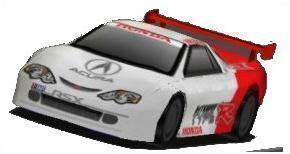
\includegraphics[scale= 0.2,type=jpg,ext=.jpg,read=.jpg]{figures/acura}\vspace{1 mm}} & Acura NSX type S-Zero & 1200 & 285 & 0.612 & Rwd\footnote{\textit{Rear Wheel Drive}, carros con tracción en las ruedas traseras.} & 5.00 & 1.92 \\ \hline

\parbox{2.5 cm}{\vspace{1 mm} 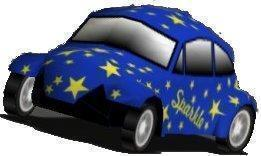
\includegraphics[scale= 0.2,type=jpg,ext=.jpg,read=.jpg]{figures/bug}\vspace{1 mm}}&Baja Bug & 600 & 82 & 0.9 & Rwd & 3.8 & 1.8 \\ \hline

\parbox{3 cm}{\vspace{1 mm} 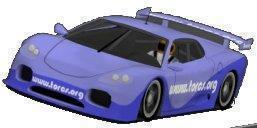
\includegraphics[scale= 0.2,type=jpg,ext=.jpg,read=.jpg]{figures/trb}\vspace{1 mm}} & Car1-trb1  & 1150 & 405 & 0.662 & Rwd & 4.52 & 1.94 \\ \hline

\parbox{2.5 cm}{\vspace{1 mm} 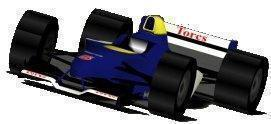
\includegraphics[scale= 0.2,type=jpg,ext=.jpg,read=.jpg]{figures/f1}\vspace{1 mm}} & sc-f1 & 650 & 677 & 0.336 & Rwd & 4.3 & 2.0 \\ \hline

\parbox{2.5 cm}{\vspace{1 mm} 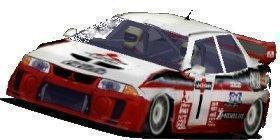
\includegraphics[scale= 0.2,type=jpg,ext=.jpg,read=.jpg]{figures/evo}\vspace{1 mm}}& Mitsubishi Lancer EVO & 900 & 321 & 0.6 & 4WD\footnote{\textit{Four Wheel Drive}, carros con tracción en las cuatro ruedas.} & 4.2 & 2.02 \\ \hline

\parbox{2.5 cm}{\vspace{1 mm} 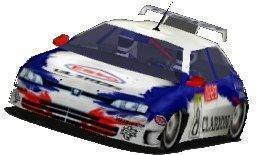
\includegraphics[scale= 0.2,type=jpg,ext=.jpg,read=.jpg]{figures/306} \vspace{1 mm}} & Peugeot 306 Maxi  & 950 & 246 & 0.77 & 4WD & 3.89 & 2.0 \\ \hline

\parbox{2.5 cm}{\vspace{1 mm} 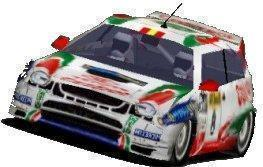
\includegraphics[scale= 0.2,type=jpg,ext=.jpg,read=.jpg]{figures/corolla}\vspace{1 mm}}& Toyota Corolla WRC  & 905 & 329 & 0.770 & 4WD & 3.81 & 1.98 \\ \hline

\end{tabular}
\caption{Tabla comparativa de los atributos de los vehículos}
\label{tab:compCar}
\end{minipage}
\end{table}

Ejecutando la simulación utilizando los siete vehículos presentados en la tabla \ref{tab:compCar}, se obtuvieron los resultados de la figura \ref{fig:7cars}. A pesar de sus diferentes dinámicas, se puede observar que el comportamiento de los siete carros es prácticamente igual, y en los casos como el que se encuentra resaltado, perteneciente a los segundos 450 y 500, los vehículos no sobrepasaron el perfil de velocidad, por mucho más de 0.5 Km/h. 

En la figura \ref{fig:31cars}, correspondiente a la simulación de los 30 carros, se observa como los grandes picos, que aparecieron en el período antes de la ejecución del aprendizaje global, disminuyeron considerablemente a medida que transcurrió la simulación. A medida que los singletons se fueron estabilizando, se fue obteniendo un mejor control y se logra disminuir la diferencia con respecto al perfil de velocidad a menos de 1 km/h, como se puede apreciar en el acercamiento realizado entre los segundos 780 y 800.   

\begin{minipage}{1\linewidth}
\end{minipage}
\begin{figure}[htb]
\centering
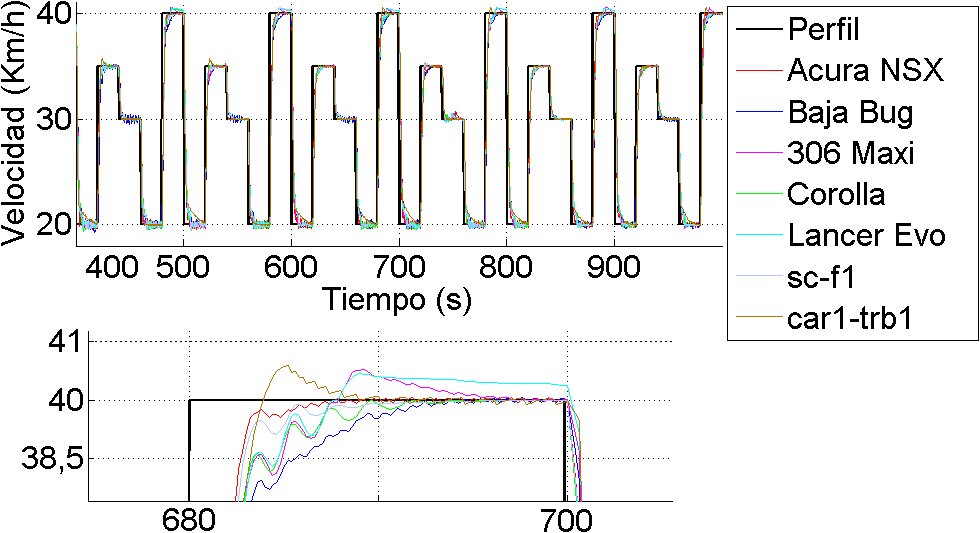
\includegraphics[width=0.6\linewidth,type=png,ext=.png,read=.png]{figures/7cars}
\caption{Velocidad de los carros entre los 400 y 1000 segundos de la ejecución de las pruebas}
\label{fig:7cars}
\end{figure}  
  
\begin{figure}[htb]
\centering
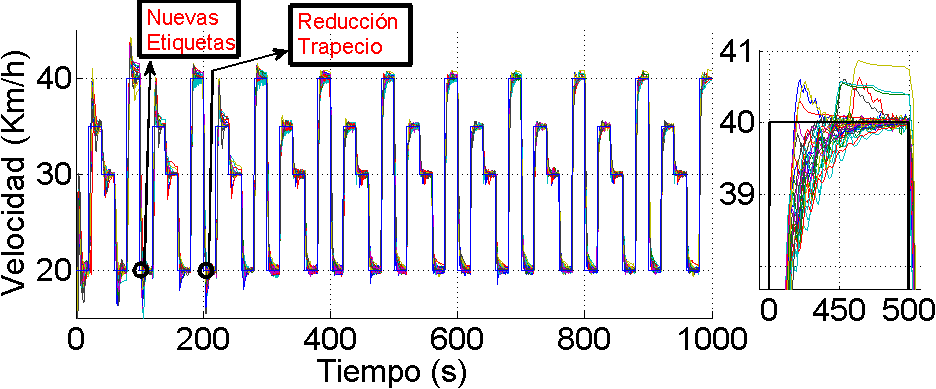
\includegraphics[width=0.6\linewidth,type=png,ext=.png,read=.png]{figures/31cars}
\caption{Velocidad de los 30 carros que corrieron la simulación.}
\label{fig:31cars}
\end{figure}


\section{Pruebas realizadas con vehículo automatizado}
\label{sec:pCampo}

Para la fase final del proyecto, se utilizó a \textbf{Platero} (sección \ref{sec:carros}) como vehículo de pruebas. Con cada prueba se buscó ajustar y mejorar el sistema, para hacerlo lo más preciso y confortable posible.

Resultados empíricos prueban que valores superiores a 0.5 sobre el acelerador producen aceleraciones muy altas sobre el vehículo, por lo que deben ser evitados con el fin de obtener un control confortable para los ocupantes del vehículo; por otra parte, valores superiores a 0.2 sobre el freno pueden producir desaceleraciones bruscas, llegando incluso a ser peligrosas \cite{Milanes2010}. Teniendo esto en cuenta, antes de comenzar con cualquier tipo de prueba, se limitó la salida correspondiente al pedal, así como los límites de los singletons, para respetar dichos valores.

Los resultados de velocidad presentados en cada experimento, se obtuvieron por medio del modulo \gls{CAN} de Platero, y poseen un error estimado de 0.1 km/h. 

\subsection{Perfil constante a 15 km/h}
\label{subsec:p15}

Para la primera prueba en Platero, se condujo el vehículo por \gls{ZOCO}, sin tener un recorrido definido, por un período de 340 segundo (1700 iteraciones), utilizando una consigna de velocidad constante a 15 Km/h. Se utilizó este valor porque es una velocidad algo complicada para el sistema, ya que la frontera del cambio automático de la transmisión entre primera y segunda es cercano a esa velocidad\footnote{No se dispone de la especificación técnica del cambio de marchas, pero se supone que dicho control no dependerá únicamente de la velocidad, lo haría también de otras variables como pueden ser las revoluciones por minuto del motor, etcétera.}, por lo que el control de velocidad se hace más inestable.

Como en los instantes iniciales de las cuatro primeras pruebas el automóvil alcanzó velocidades cercanas a los 20 km/h, se activó el cambio automático de la caja de velocidades de primera a segunda. Como parte de la prueba, se decidió en el segundo 300 (equivalente a 1500 iteraciones) reducir la velocidad de la caja de segunda a primera, manteniendola así hasta finalizar la prueba, de manera que se pudiera observar como el vehículo se adaptaba al nuevo cambio. En las dos últimas pruebas no se llegaron a  alcanzar velocidades muy por encima de 15 km/h, por lo que no se activó el cambio automático de primera a segunda, manteniendo la trasmisión en primera durante el transcurso de la prueba; se intentó la opción de hacer el cambio manual, pero el vehículo no lo permitió debido a la baja velocidad a la que circulaba. 

Para medir la eficacia del sistema, se calculó el \gls{MAE}, el cual se puede observar en la leyenda de cada figura correspondiente a la velocidad de los vehículos. En este caso como no no se realizaron variaciones en el perfil de velocidad, el \gls{MAE}, resulta un buen indicador para medir el funcionamiento del controlador.

Entre cada prueba realizada, se fueron modificando los atributos del controlador, con el fin de encontrar la configuración que otorgase el mejor desempeño. Las configuraciones utilizadas en cada prueba son presentadas en la tabla \ref{tab:compCar}.

\begin{table}[!h]
\centering
\begin{tabular}{|c|c|c|c|}
\hline 
\rowcolor[gray]{0.9} Prueba &  $Cte$ & Rango & Etiquetas\\
\hline \hline 
0  & 100 & \parbox[t]{3cm} {\hspace{8 px} $\varepsilon=[-20,20]$ \\ $\frac{d(\varepsilon)}{d(t)}=[-8,8]$ \vspace{1mm}} &  \parbox[t]{3cm} {\hspace{11 px}$\varepsilon=2$\\ $\frac{d(\varepsilon)}{d(t)}=2$} \\ 
\hline 

1 & 100 & \parbox[t]{3cm} {\hspace{8 px} $\varepsilon=[-20,20]$ \\ $\frac{d(\varepsilon)}{d(t)}=[-5,5]$} &  \parbox[t]{3cm} {\hspace{11 px}$\varepsilon=2$\\ $\frac{d(\varepsilon)}{d(t)}=2$} \\ 
\hline 

2 & 200 & \parbox[t]{3cm} {\hspace{8 px} $\varepsilon=[-20,20]$ \\ $\frac{d(\varepsilon)}{d(t)}=[-5,5]$} &  \parbox[t]{3cm} {\hspace{11 px}$\varepsilon=2$\\ $\frac{d(\varepsilon)}{d(t)}=2$} \\ 
\hline 

3 & 100 & \parbox[t]{3cm} {\hspace{8 px} $\varepsilon=[-10,10]$ \\ $\frac{d(\varepsilon)}{d(t)}=[-5,5]$} &  \parbox[t]{3cm} {\hspace{11 px}$\varepsilon=2$\\ $\frac{d(\varepsilon)}{d(t)}=2$} \\ 
\hline 

4 & 100 & \parbox[t]{3cm} {\hspace{8 px} $\varepsilon=[-20,20]$ \\ $\frac{d(\varepsilon)}{d(t)}=[-5,5]$} &  \parbox[t]{3cm} {\hspace{11 px}$\varepsilon=4$\\ $\frac{d(\varepsilon)}{d(t)}=2$} \\ 
\hline

5 & 100 & \parbox[t]{3cm} {\hspace{8 px} $\varepsilon=[-20,20]$ \\ $\frac{d(\varepsilon)}{d(t)}=[-5,5]$ \\ $perfil=[0,40]$} &  \parbox[t]{3cm} {\hspace{11 px}$\varepsilon=4$\\ $\frac{d(\varepsilon)}{d(t)}=2$\\$perfil=2$} \\ 
\hline  
\end{tabular}
\caption{Comparación entre los parámetros de las pruebas realizadas con un perfil de velocidad constante a 15 km/h}
\label{tab:comparacionPruebas}
\end{table}



\begin{figure}[h]
\centering
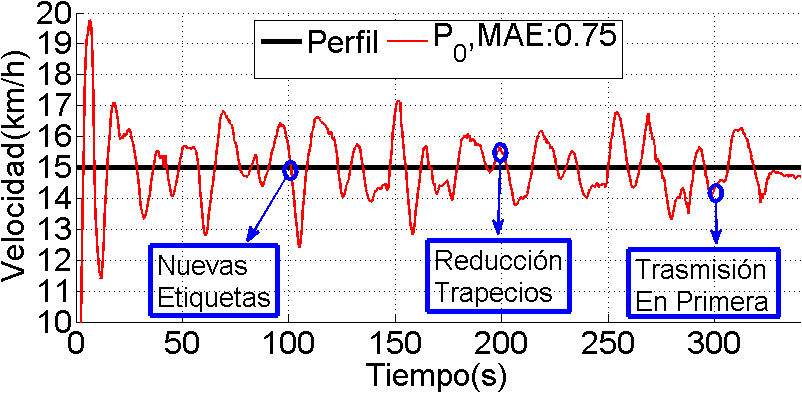
\includegraphics[width=0.45\linewidth]{figures/p0.png}\hspace{0.5cm}
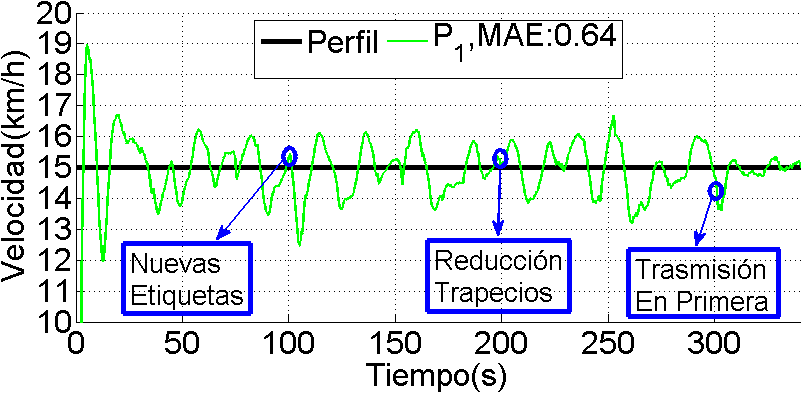
\includegraphics[width=0.45\linewidth]{figures/p1.png}\\
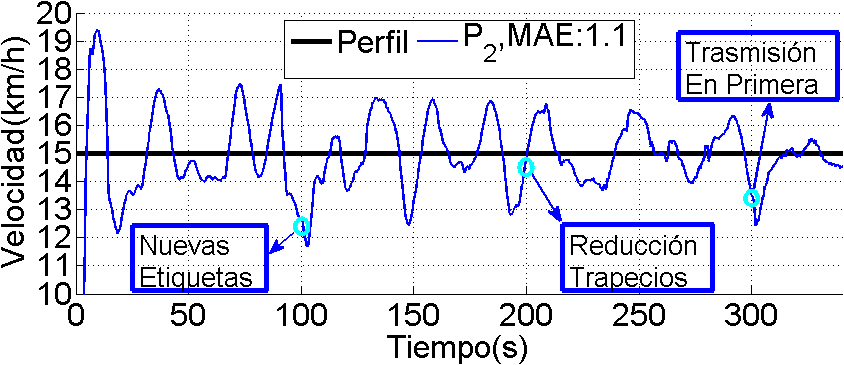
\includegraphics[width=0.45\linewidth]{figures/p2.png}\hspace{0.5cm}
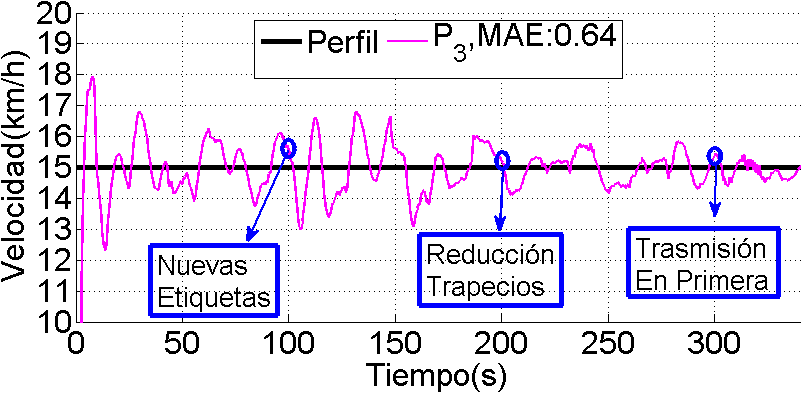
\includegraphics[width=0.45\linewidth]{figures/p3.png}\\
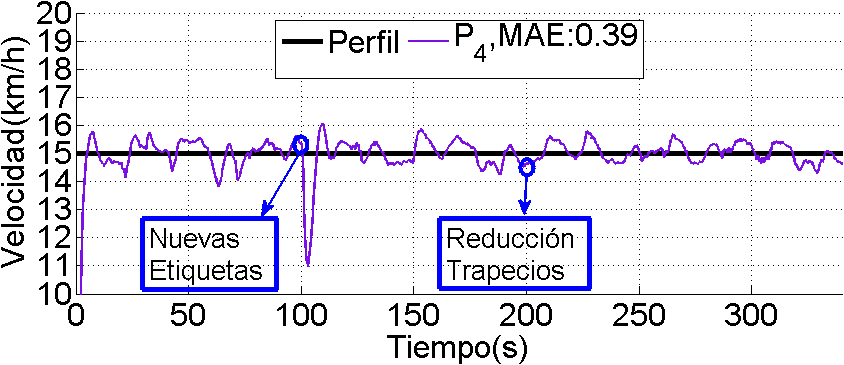
\includegraphics[width=0.45\linewidth]{figures/p5.png}\hspace{0.5cm}
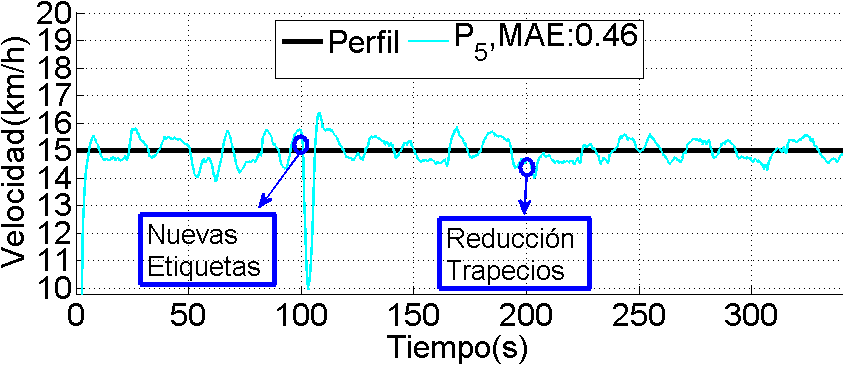
\includegraphics[width=0.45\linewidth]{figures/final15.png}
\caption{Velocidad del vehículo durante las pruebas a 15 km/h. Prueba 0 (arriba izquierda), Prueba 1 (arriba derecha), Prueba 2 (centro izquierda), Prueba 3 (centro derecha), Prueba 4 (abajo izquierda) y Prueba 5 (abajo derecha)}
\label{fig:pruebas15}
\end{figure}


En la figura \ref{fig:pruebas15}, se muestran los resultados obetidos en las cinco pruebas realizadas a 15 km/h. La \textbf{prueba 0} (figura \ref{fig:pruebas15} arriba izquierda) se realizó para comprobar que el sistema funcionara correctamente al ser adaptado al programa de control del vehículo. La configuración utilizada durante la ejecución no varió mucho de la utilizada con \gls{TORCS}, solo se redujo el rango del error a [-20,20]. No ocurrió ningún percance durante la ejecución de la prueba. Exceptuando los primero instantes cuando tiene que pasar de 0 km/h a 15 km/h, la diferencia entre la velocidad del automóvil y el perfil de velocidad, no llega a ser superior a los 3 km/h. 

En la \textbf{prueba 1} (figura \ref{fig:pruebas15} arriba derecha) se observa una pequeña mejora con respecto a la \textit{prueba 0}, debido a que se redujo el rango de la derivada del error de velocidad a [-5,5], con lo que se logró disminuir el \gls{MAE} a 0.64, y se redujeron un poco el tamaño de las oscilaciones.

Se aumentó la constante de normalización de 100 a 200 en la \textbf{prueba 2} (figura \ref{fig:pruebas15} centro izquierda), para intentar disminuir la magnitud de los cambios de los singletons, y buscar disminuir las oscilaciones con respecto al perfil de velocidad. Con esta configuración se obtuvieron los peores resultados, las oscilaciones fueron muy grandes, y se alcanzaron diferencias con respecto a la velocidad deseada superiores a 2 km/h. Se obtuvo un \gls{MAE} de 1.1, el cual fue el más elevado que se obtuvo entre todas las pruebas.

Tomando en cuenta los malos resultados de la \textit{prueba 2}, se retomó la constante de normalización con un valor de 100 para la \textbf{prueba 3} (figura \ref{fig:pruebas15} centro derecha). Aunque obtuvo un \gls{MAE} de 0.64, al igual que la \textit{prueba 1}, se observa que a partir del segundo 200, la velocidad del vehículo logró estabilizarse un poco, reduciendo el tamaño de las oscilaciones. En la \textit{prueba 1}, las oscilaciones solo parecen reducirse, en el segundo 300, cuando se bajó la caja de cambio de segunda a primera.    

En estas cuatro primeras pruebas, al realizar el cambio en la transmisión velocidad de segunda a primera, resulto más fácil para el vehículo mantener una velocidad cercana a los 15 km/h, logrando que las oscilaciones disminuyeran considerablemente.

La primera prueba que no realizó el gran salto en velocidad que presentaron las anteriores al pasar de 0 km/h a 15 km/h fue la \textbf{prueba 4} (figura \ref{fig:pruebas15} abajo izquierda), esto se debe a que se utilizaron cuatro etiquetas para el error de velocidad en vez de dos. Esta configuración obtuvo los mejores resultados, logrando el mínimo \gls{MAE}. La única oscilación grande que se puede apreciar, se encuentra luego del segundo 100, que es el instante cuando se ejecuta el aprendizaje global y se reinician los singletons; pero luego al estabilizarse, la diferencia entre la velocidad del perfil y la velocidad del carro, ni siquiera llega a ser 1 km/h. Esta y la siguiente prueba se realizaron con la transmisión en primera velocidad durante toda la ejecución, ya que el controlador nunca revolucionó lo suficiente como para permitir hacer el cambio manual.

En la \textbf{prueba 5} (figura \ref{fig:pruebas15} arriba derecha) \textbf{se agregó el valor del perfil de velocidad como tercera variable de entrada}, con la finalidad de lograr un mejor control al momento de mantener la velocidad constante. Desde el punto de vista del pedal, no implica lo mismo mantener al vehículo constante a una velocidad u otra, la variable de entrada adicional permite marcar esta diferencia y controlar mejor cada caso que pueda presentarse. Aunque los resultados fueron muy buenos, no llegaron a ser mejores que los de la \textit{prueba 4}, ya que obtuvo un \gls{MAE} un poco mayor.

 
\subsubsection*{Comparación entre conducción automática y conductor humano}
\label{subsec:autoManual}

Para comparar el desempeño del sistema con la manera de manejar de un persona, se hizo una prueba en la que no se activó el control de conducción automática, sino que se manejó manualmente durante el mismo periodo de tiempo que duraron las pruebas, intentando mantener la velocidad constante a 15 km/h.    

\begin{figure}[!h]
\centering
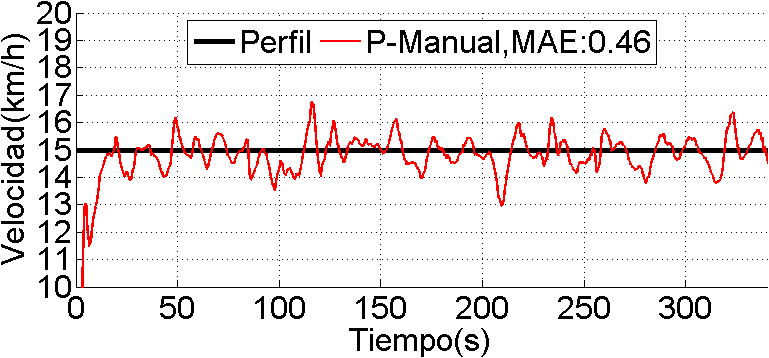
\includegraphics[width=0.6\linewidth]{figures/manual.png}
\caption{Velocidad del automóvil conducido de forma manual.}
\label{fig:manual}
\end{figure}

Como se observa en la figura \ref{fig:manual} se obtuvieron mejores resultados utilizando la configuración de la \textit{prueba 4}, que la persona que condujo el carro durante la prueba manual, lo cual se ve reflejado en el \gls{MAE}; en la prueba manual fue de 0.46, y en la \textit{prueba 4} fue de 0.39. Se debe tener en cuenta que la reinicialización de los singletons contribuyeron al aumento del \gls{MAE} en las pruebas, porque en ese instante ocurrió una reducción muy significativa de la velocidad, debido a que el vehículo comenzó desde cero el proceso de aprendizaje.

\subsection{Variando el perfil a lo largo de la ejecución}
\label{subsec:variandoP}

Debido a los buenos resultados obtenidos con la configuración de la \textit{prueba 4}, se seleccionó dicho modelo para realizar una prueba en la cual vamos a ir variando el perfil de velocidad. De esta manera se  analizó la forma en que se adaptó el aprendizaje del controlador a los constantes cambios en la consigna de velocidad.

\begin{figure}[htb]
\centering
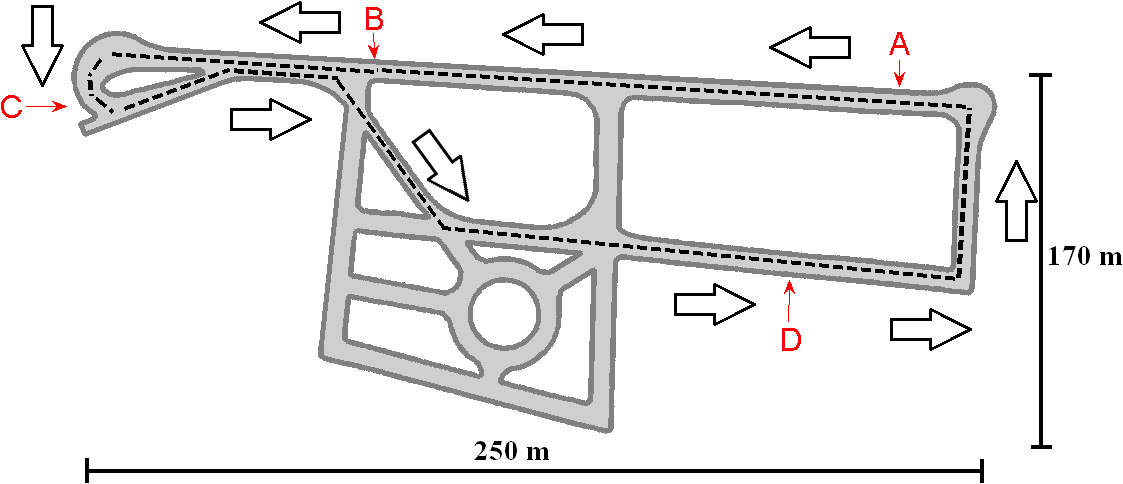
\includegraphics[width=0.6\linewidth, height = 3cm]{figures/zoconp6.png}
\caption{Recorrido utilizado para la prueba con variación en el perfil de velocidad.}
\label{fig:zoconp6}
\end{figure}

La prueba se realizó circulando por el recorrido que se muestra en la figura \ref{fig:zoconp6}, partiendo del punto \textit{A}. Los cambios en el perfil se van a realizar en los puntos marcados en el mapa de la pista, el tramo entre el punto \textbf{B} y el punto \textbf{C} consiste en una pendiente que presenta un desnivel de aproximadamente 2\%, mientras que el resto de la pista no presenta mayores diferencias de elevación. Debido al reducido tamaño de la pista, la velocidad máxima a la que se llegó el vehículo fue 40 km/h.

En la figura \ref{fig:pPerfil} se puede observar la velocidad del controlador con respecto al perfil de velocidad que se utilizó a lo largo de la prueba. A simple vista se observa que el sistema tuvo un desempeño muy bueno, no se observan diferencias muy grandes con respecto al perfil. La figura \ref{fig:v1} se ve con detalle los resultados correspondientes a la velocidad y se especifica los puntos de la pista por los que pasaba el vehículo.

%\begin{figure}[htb]
%\centering
%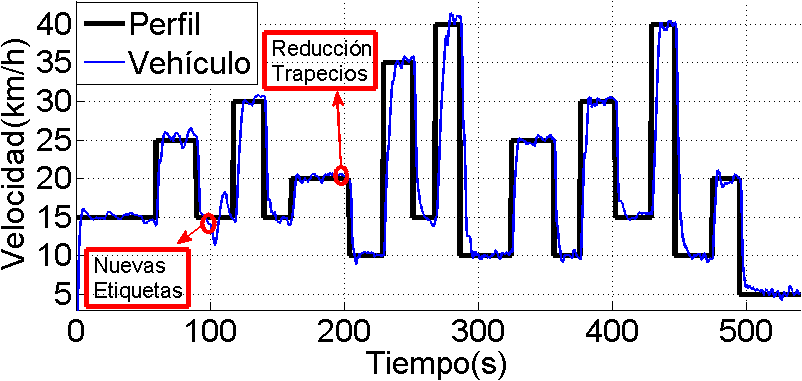
\includegraphics[width=0.6\linewidth]{figures/p6.png}
%\caption{Velocidad del vehículo durante la prueba con variación en el perfil de velocidad.}
%\label{fig:pPerfil}
%\end{figure}

Durante la primera vuelta no se modificó el perfil hasta que se llegó al punto \textbf{C} como puede apreciarse en la figura \ref{fig:v1} (arriba), ya que se utilizó el tramo \textbf{A-C} para que el controlador se adaptase lo mejor posible antes de realizar el primer cambio.

\begin{figure}[htb]
\centering
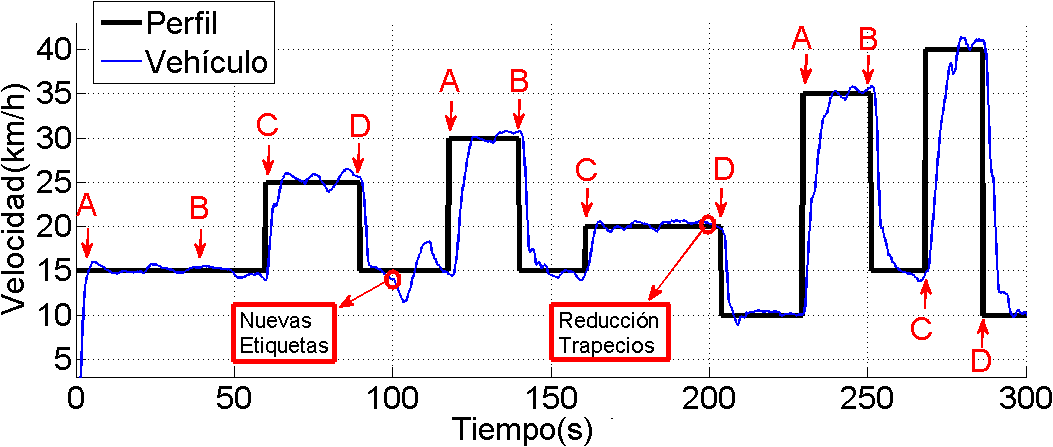
\includegraphics[width=0.65\linewidth]{figures/p61.png}
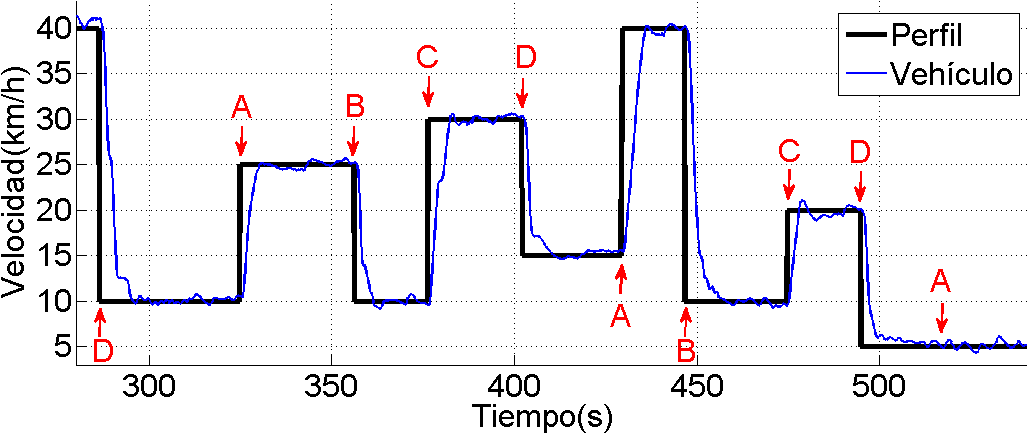
\includegraphics[width=0.65\linewidth] {figures/p62.png}
\caption{Velocidad del vehículo indicando los puntos de la pista por los que pasa el vehículo, durante la prueba con variación en el perfil de velocidad. Primera mitad (izquierda), segunda mitad (derecha).}
\label{fig:v1}
\end{figure}

Desde el comienzo de la prueba hasta que llegamos al punto \textbf{D}, no se observa una diferencia muy grande entre la velocidad deseada y la velocidad real del vehículo; a diferencia del tramo siguiente, en el que luego del segundo 100, nos encontramos con diferencias de hasta 3 km/h. La variación en la velocidad, se debe a que en ese instante de tiempo se activó el aprendizaje global y se reiniciaron los singletons del controlador. En la segunda mitad de la prueba (figura \ref{fig:v1} abajo), el vehículo se comportó de manera excepcional, ajustándose a los cambios de velocidad sin ningún problema.

\definecolor{bb}{RGB}{99,184,255}
\begin{table}[htb]
\centering
\begin{minipage}{\linewidth}
\begin{tabular}{|c|c|c|c|c|c|}
\hline 
\rowcolor[gray]{0.9} \parbox[t]{2cm}{\textbf{Tramo km/h}}& \parbox[t]{2cm}{\textbf{Aceleración\\Media km/h/s}\vspace{1mm}} & \parbox[t]{2cm}{\textbf{Aceleración \\en $V_p$ $\pm 0.5$ km/h/s}} & \parbox[t]{2cm}{\textbf{Error\\ Medio km/h}} & \parbox[t]{2cm}{\textbf{Error\\ Máximo km/h}} & \parbox[t]{2cm}{\textbf{Error\\ Mínimo km/h}} \\ 
\hline \hline 
0-15 & 6.82 & 8.67 & 0.36 & 1.08 & -1.01 \\ 
\hline 
15-25 & 6.25 & 4.66 & 0.66 & 1.53 & -1.05 \\ 
\hline 
25-15 & \cellcolor{bb}  -5.56 & -4.79 & 1.39 & 3.27 & -3.56 \\ 
\hline 
15-30 & 3.26 & 2.61 & 0.42 & 0.79 & -1.09 \\ 
\hline 
30-15 & \cellcolor{bb} -6.25 & -7.38 & 0.48 & 0.72 & -1.09 \\ 
\hline 
15-20 & *\footnote{La aceleración media se midió hasta que se alcanza la velocidad de la consigna más o menos 5 km/h, por lo que no se pudo calcular en este caso.} & 0.61 & 0.36 & 0.68 & -0.70 \\ 
\hline 
20-10 &\cellcolor{bb} -6.25 & -5.12 & 0.29 & 0.55 & -1.12 \\ 
\hline 
10-35 & 4.63 & 2.81 & 0.37 & 0.79 & -0.71 \\ 
\hline 
35-15 &\cellcolor{bb} -7.14 & -8.42 & 0.52 & 0.56 & -1.18 \\ 
\hline 
15-40 & 4.03 & 2.09 & 0.79 & 1.40 & -0.80 \\ 
\hline 
40-10 &\cellcolor{bb} -6.82 & -7.85 & 0.24 & 0.75 & -0.41 \\ 
\hline 
10-25 & 5.77 & 4.26 & 0.32 & 0.67 & -0.67 \\ 
\hline
25-10 &\cellcolor{bb} -8.33 & -9.21 & 0.30 & 0.76 & -0.85 \\ 
\hline
10-30 & 4.55 & 1.81 & 0.34 & 0.60 & -0.68 \\ 
\hline
30-15 &\cellcolor{bb} -8.33 & -8.85 & 0.36 & 0.66 & -0.36 \\ 
\hline
15-40 & 5.43 & 4.34 & 0.37 & 0.46 & -0.86 \\ 
\hline
40-10 &\cellcolor{bb} -7.50 & -5.62 & 0.29 & 0.94 & -0.79 \\ 
\hline
10-20 & 6.25 & 3.70 & 0.57 & 1.07 & -1.14 \\ 
\hline
20-5 &\cellcolor{bb} -7.50 & -8.84 & 0.36 & 1.11 & -0.70 \\ 
\hline
\end{tabular}
\end{minipage} 
\caption{Valores correspondientes a los tramos de cambio de velocidad}
\label{tab:p6}
\end{table}

En la tabla \ref{tab:p6} se presentan valores correspondientes a la aceleración y velocidad obtenidos durante la prueba. \textbf{La aceleración media} se midió desde el momento en que ocurre un cambio de perfil, hasta que se alcanza la velocidad del perfil más o menos 5 km/h; \textbf{la aceleración en $V_p\pm0.5$} corresponde a la aceleración cuando se reduce a $\pm0.5$ km/h el error de velocidad entre el vehículo y el perfil, justo después de ocurrir un cambio en la consigna. 

Los valores que están resaltados en azul en la tabla \ref{tab:p6}, corresponden a la aceleración media en los tramos donde el carro se encontraba frenando, dichos valores presentan tendencia hacia los -8km/h/s, por lo que se puede decir que la aceleración media cuando el vehículo desacelera es aproximadamente igual a la aceleración de confort; en cambio cuando el automóvil acelera, la aceleración media tiende a 4 km/h/s, lo que es equivalente a la mitad de la aceleración de confort. La discrepancia en la tendencia de la aceleración media en ambos casos, indica que el efecto del pedal de freno sobre el estado del vehículo influye de mayor manera que el pedal del acelerador.  

\textbf{El error medio, error máximo y error mínimo}, se calcularon a partir del punto en que se alcanza $V_p\pm0.5$, hasta que ocurrió un cambio en el perfil de velocidad. Únicamente en el tercer tramo, el cual va de 25 a 15 km/h, el error medio fue mayor a 1 km/h; esto gracias a que en este tramo se insertaron nuevas etiquetas a las variables de entrada y se reinicializaron los singletons. En general los errores máximos y mínimos son muy bajos, encontrándose la mayoría al rededor de $\pm 1$ km/h.

Teniendo en cuenta que los velocímetros analógicos, tienen una precisión de 10 km/h, y tanto estos como los digitales  no son completamente exactos,  podemos decir que los valores obtenidos en esta prueba son muy favorables, y la diferencias de velocidad entre el vehículo y el perfil, resulta casi imperceptible para el conductor. 
\begin{figure}[htb]
\centering
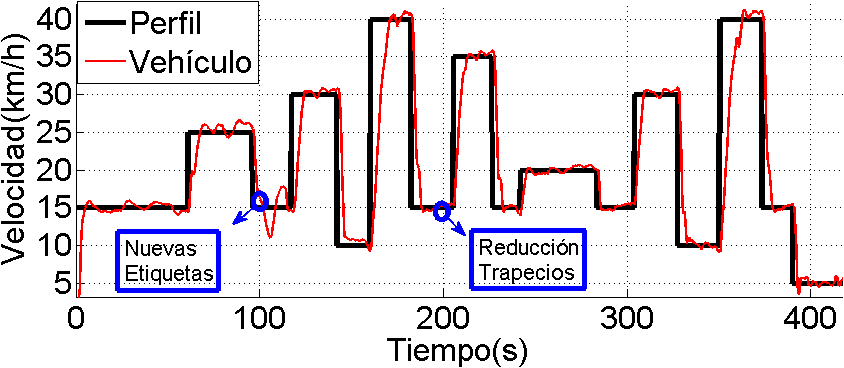
\includegraphics[width=0.6\linewidth]{figures/finalcambios.png}
\caption{Resultado de prueba cambiando el perfil de velocidad, utilizando controlador con tres variables de entrada}
\label{fig:finalcambios}
\end{figure}

\begin{table}[htb]
\centering
\begin{tabular}{|c|c|c|c|}
\hline 
\rowcolor[gray]{0.9} \textbf{Configuración} & \parbox[t]{3.5cm}{\textbf{Media del error medio km/h}} & \parbox[t]{3.5cm}{\textbf{Media del error máximo km/h}} & \parbox[t]{3.5cm}{\textbf{Media del error mínimo km/h}} \\ 
\hline \hline 
\parbox[t]{3.5cm}{Prueba 4 (dos variables entradas)}& 0.36 & 1.11 & -0.70 \\ \hline
\parbox[t]{3.5cm}{Prueba 5 (tres variables entradas)} & 0.39 & 1.67 & -1.45 \\ \hline
\end{tabular}
\caption{Tabla comparativa de las medias de los errores entre configuración con dos variables de entrada y tres variables de entrada.}
\label{tab:medias}
\end{table}

En el tabla \ref{tab:medias}, se comparan las medias de los errores, medio, máximo y mínimo, correspondientes a la configuración de tres variables de entrada, con las medias de los resultados obtenidos utilizando la configuración de 2 variables de entrada, que se presentan en la tabla \ref{tab:p6}. Como se puede observar, la diferencia de la media del error medio entre los dos es muy pequeña, pero la diferencia entre los errores mínimos y máximos de cada uno es notable; con la media del error mínimo de la configuración de tres variables de entrada llegando a ser el doble de la de dos variables, lo que indica que aunque la diferencia no es mucha, no hay mejora utilizando tres variables de entrada.  

\subsection{Comparación entre conducción automática y conducto humano a una velocidad constante de 5 km/h}

%Comparación entre conducción automática y conducción manual realizada por una persona a una velocidad constante de 5 km/h

Para probar que tan preciso puede llegar a ser el sistema en un caso extremo, se realizó una nueva comparación entre la capacidad de una persona contra la del sistema de mantener la velocidad del vehículo constante, pero a una velocidad de a 5 km/h. Se eligió un valor muy pequeño, porque a esa velocidad los efectos del pedal y las diferencias de elevación de la pista, por muy pequeñas que sean, causan un mayor impacto en la aceleración del vehículo; de manera tal, que mantener la velocidad casi constante, se convierta en una tarea muy complicada. Se configuró el sistema de la misma manera que en la \textit{prueba 4} de la sección \ref{subsec:p15}, ya que fue la que obtuvo los mejores resultados.

\begin{figure}[htb]
\centering
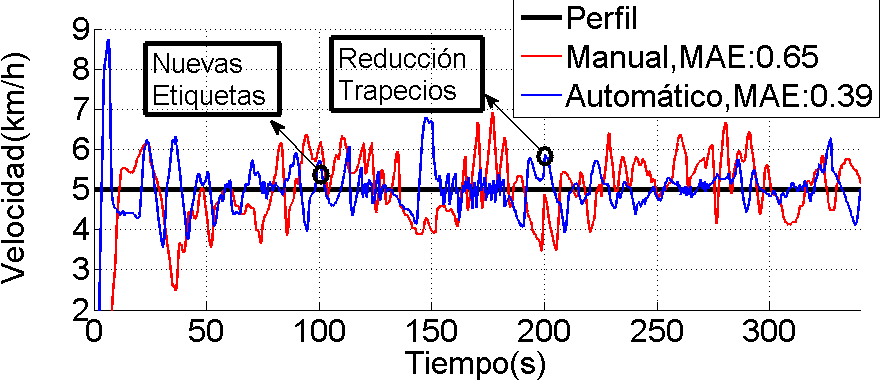
\includegraphics[width=0.6\linewidth]{figures/AutoVsManual.png}
\caption{Comparación entre un vehículo conducido de forma manual, contra uno con conducción automática, ambos a una velocidad constante a 5 km/h.}
\label{fig:autoVsmanual}
\end{figure}

Como se puede ver en la figura \ref{fig:autoVsmanual}, el sistema de conducción automática obtuvo mejores resultados que el conductor humano. Aunque casi llega al doble de la velocidad esperada en los primeros instantes, el sistema obtuvo un \gls{MAE} mucho menor al de la persona.

En el segundo 150 de la prueba, se puede observar que el sistema casi llega a los 7 km/h, esto se debe a que el aprendizaje global se ejecutó justo un poco antes de comenzar la pendiente en bajada, por lo que el controlador tardó un poco más de tiempo en estabilizarse, luego de eso el controlador logra mantenerse muy cerca de la velocidad deseada, lo cual ocurre al empezar a subir por la pendiente de la pista. Durante el transcurso de la prueba, el velocímetro digital que posee el vehículo, se mantuvo en cero, y solo algunas veces, indicaba que íbamos a una velocidad de 5 o 6 km/h.   